\documentclass[a4paper, 12pt]{article}
\usepackage[a4paper,top=1.5cm, bottom=1.5cm, left=1cm, right=1cm]{geometry}
\usepackage{cmap}					
\usepackage{mathtext} 				
\usepackage[T2A]{fontenc}			
\usepackage[utf8]{inputenc}			
\usepackage[english,russian]{babel}
\usepackage{multirow}
\usepackage{graphicx}
\usepackage{wrapfig}
\usepackage{tabularx}
\usepackage{float}
\usepackage{longtable}
\usepackage{hyperref}
\hypersetup{colorlinks=true,urlcolor=blue}
\usepackage[rgb]{xcolor}
\usepackage{amsmath, amsfonts, amssymb, amsthm, mathtools} 
\usepackage{icomma} 
\usepackage{euscript}
\usepackage{mathrsfs}
\usepackage{enumerate}
\usepackage{caption}
\usepackage{enumerate}
\mathtoolsset{showonlyrefs=true}
\usepackage{graphicx}
\usepackage{caption}
\usepackage{subcaption}
\usepackage{amsthm}
\usepackage{floatflt}
\usepackage[europeanresistors, americaninductors]{circuitikz}
\DeclareMathOperator{\sgn}{\mathop{sgn}}
\newcommand*{\hm}[1]{#1\nobreak\discretionary{}
	{\hbox{$\mathsurround=0pt #1$}}{}}

\title{\textbf{Длинные линии (3.7.3)}}
\author{Манро Эйден}
\date{}

\begin{document}

\maketitle

\noindent \textbf{Цель работы:} Ознакомится и проверить на практике теорию распространения
электрических сигналов вдоль длинной линии; измерить амплитудо- и фазово-частотные
характеристики коаксиальной линии; определить погонные характеристики такой
линии; на примере модели длинной линии изучить вопрос распределения амплитуды
колебаний сигнала по длине линии.

\bigskip

\noindent \textbf{В работе используются:} осциллограф АКТАКОМ ADS-6142H; генератора АКИП 3420/1; бухта с коаксиальным кабелем pk 50-4-11; 
	схематический блок "модель длинной линии"; магазин сопротивления Р33, соединительные провода.



 \subsection*{Экспериментальная установка}
   \begin{wrapfigure}{hr}{0.5\textwidth}
  \vspace{-20pt}
  \begin{center}
    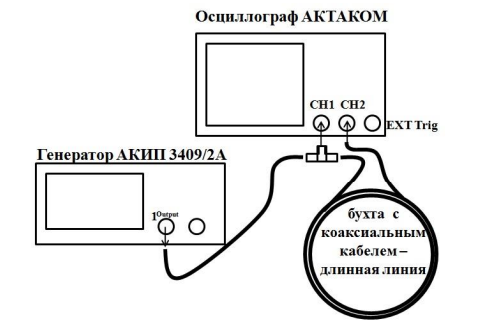
\includegraphics[width=0.5\textwidth]{ust.png}
    \caption{Схема экспериментальной установке}
  \end{center}
  \vspace{-10pt}
\end{wrapfigure}
 	Коаксиальный кабель подключается к генератору и осциллографу. На канал 1 выводится сигнал, подаваемый генератором, а с канала 2 снимается напряжение на нагрузке. Схема экспериментальной установки изображена ниже.
  
\section*{Формулы}

\begin{align*}
    V_{\text{ф}} &= \frac{f_0}{n} l & \quad L_xC_x &= \frac{c^2}{{V_{\text{ф}}}^2} \\
    L_x &= cR_0\sqrt{L_xC_x} & \quad C_x &= \frac{\sqrt{L_xC_x}}{cR_0} \\
   \varepsilon &= 2Cln\left(\frac{r_2}{r_1}\right) & \quad \mu &= \frac{L}{2ln\left(\frac{r_2}{r_1}\right)} \\
    \sigma &= \left( \frac{2C_xV_{\text{ф}}}{c \cdot d \cdot \frac{\alpha}{\sqrt{f}}} \right)^2 
\end{align*}



\section*{Результаты}

\begin{figure}[H]
    \captionsetup{position=above, skip=2pt}
    \centering
    \caption{Зависимость резонансной частоты от её номера.}
    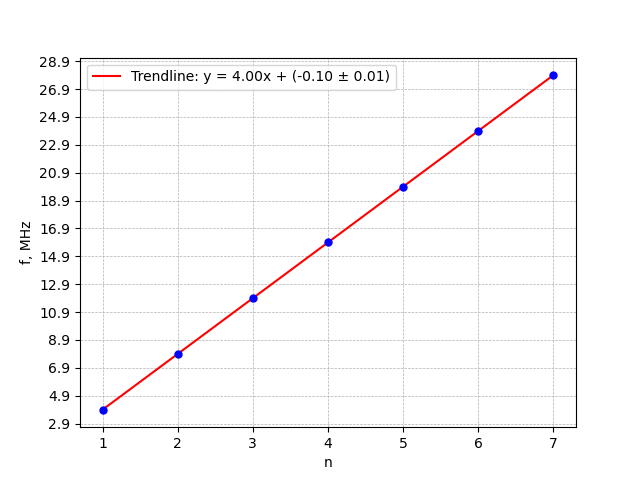
\includegraphics[width=0.9\textwidth]{fig1.png}
\end{figure}

Погонные характеристики кабеля:

$$ C_x = (1.00 \pm 0.01) \; \text{ед. СГС} $$

$$ L_x = (2.25 \pm 0.02) \; \text{ед. СГС} $$

Диэлектрическая проницаемость:

$$ \varepsilon = 2.25 \pm 0.29 $$

Магнитная восприимчивость:

$$ \mu = 1.00 \pm 0.15 $$


\begin{figure}[H]
    \captionsetup{position=above, skip=2pt}
    \centering
    \caption{Зависимость декремента затухания частоты от корня частоты гармонического сигнала.}
    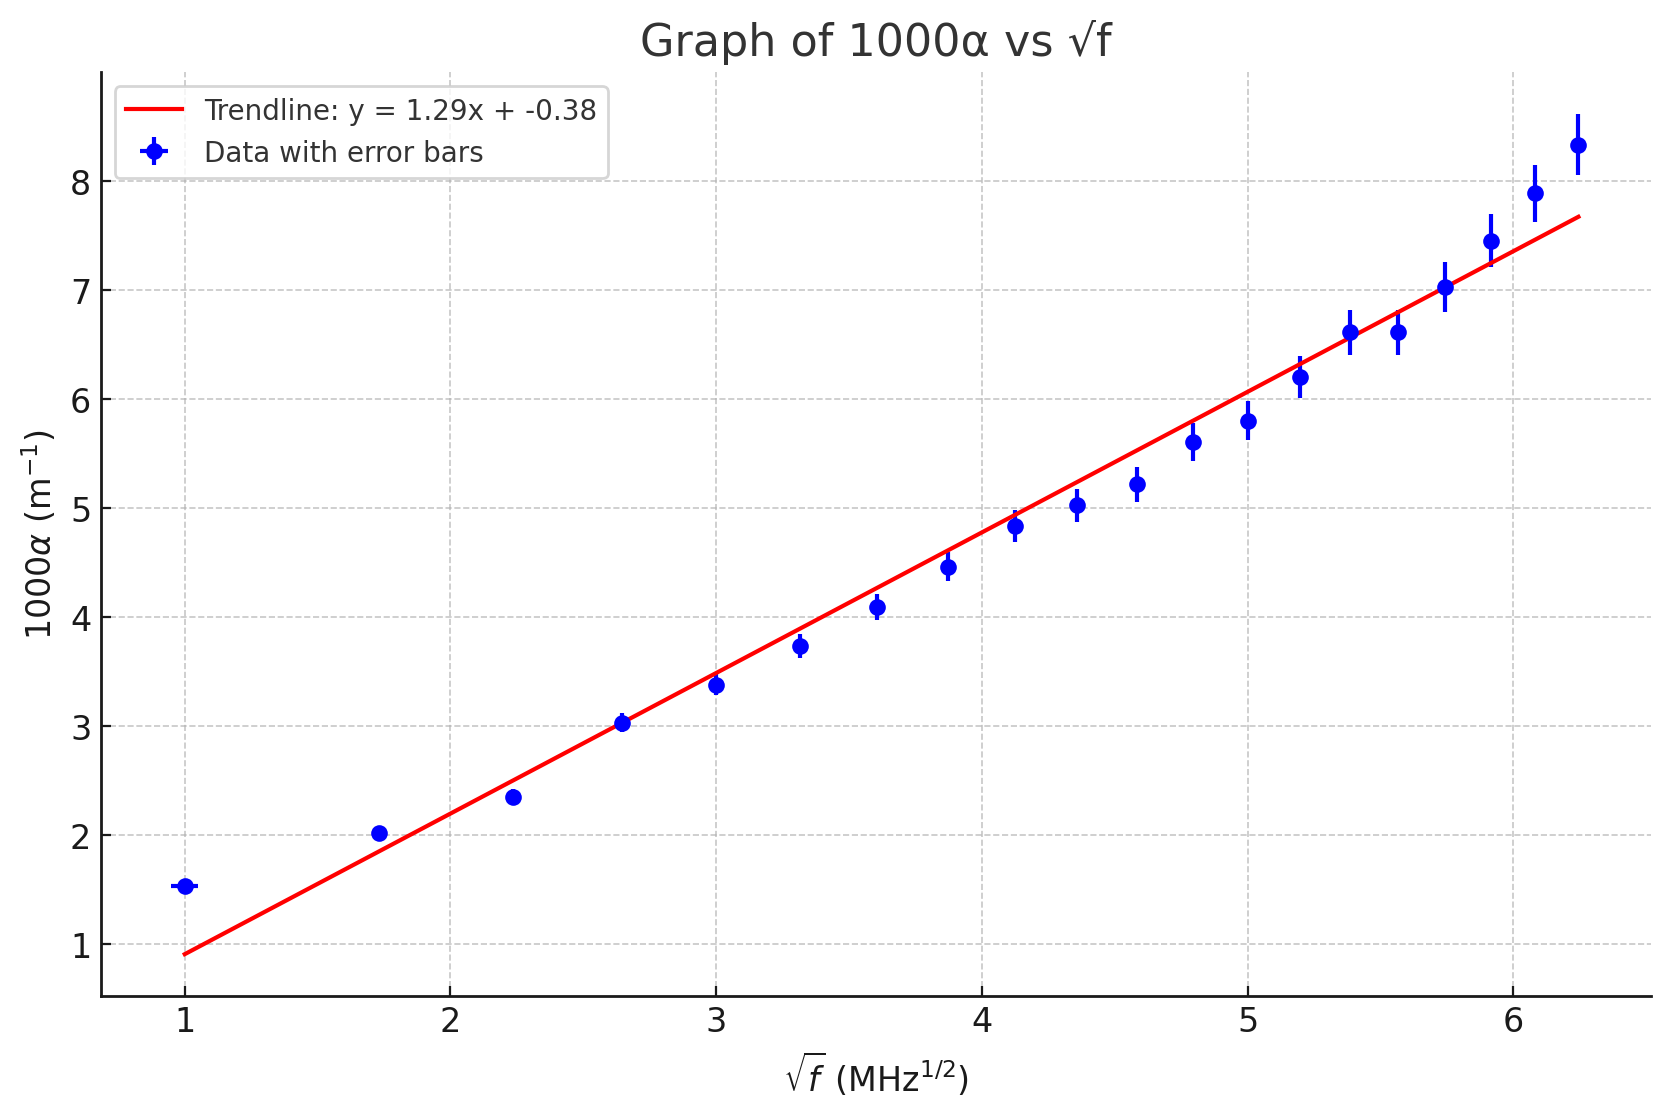
\includegraphics[width=0.9\textwidth]{fig2.png}
\end{figure}

Удельная проводимость провода:

$$ \sigma = (6.3 \pm 0.2) \; \text{ед. СГС} $$

\section*{Вывод}

 В ходе работы были изучены основные характеристики коаксиальной линии и проведены измерения для определения её погонных параметров. Фазовые скорости в условиях согласованной нагрузки и при отсутствии нагрузки совпадают для любого сигнала. Несмотря на некоторые искажения на малых и больших частотах на графике декремента затухания, данные находятся в пределах ожидаемой погрешности, что является нормой для измерений вблизи граничных частот. Также 


\end{document}